\documentclass[tikz,border=12pt]{standalone}
\usepackage{tikz}
\usetikzlibrary{arrows.meta,positioning,fit,backgrounds,calc}

\begin{document}
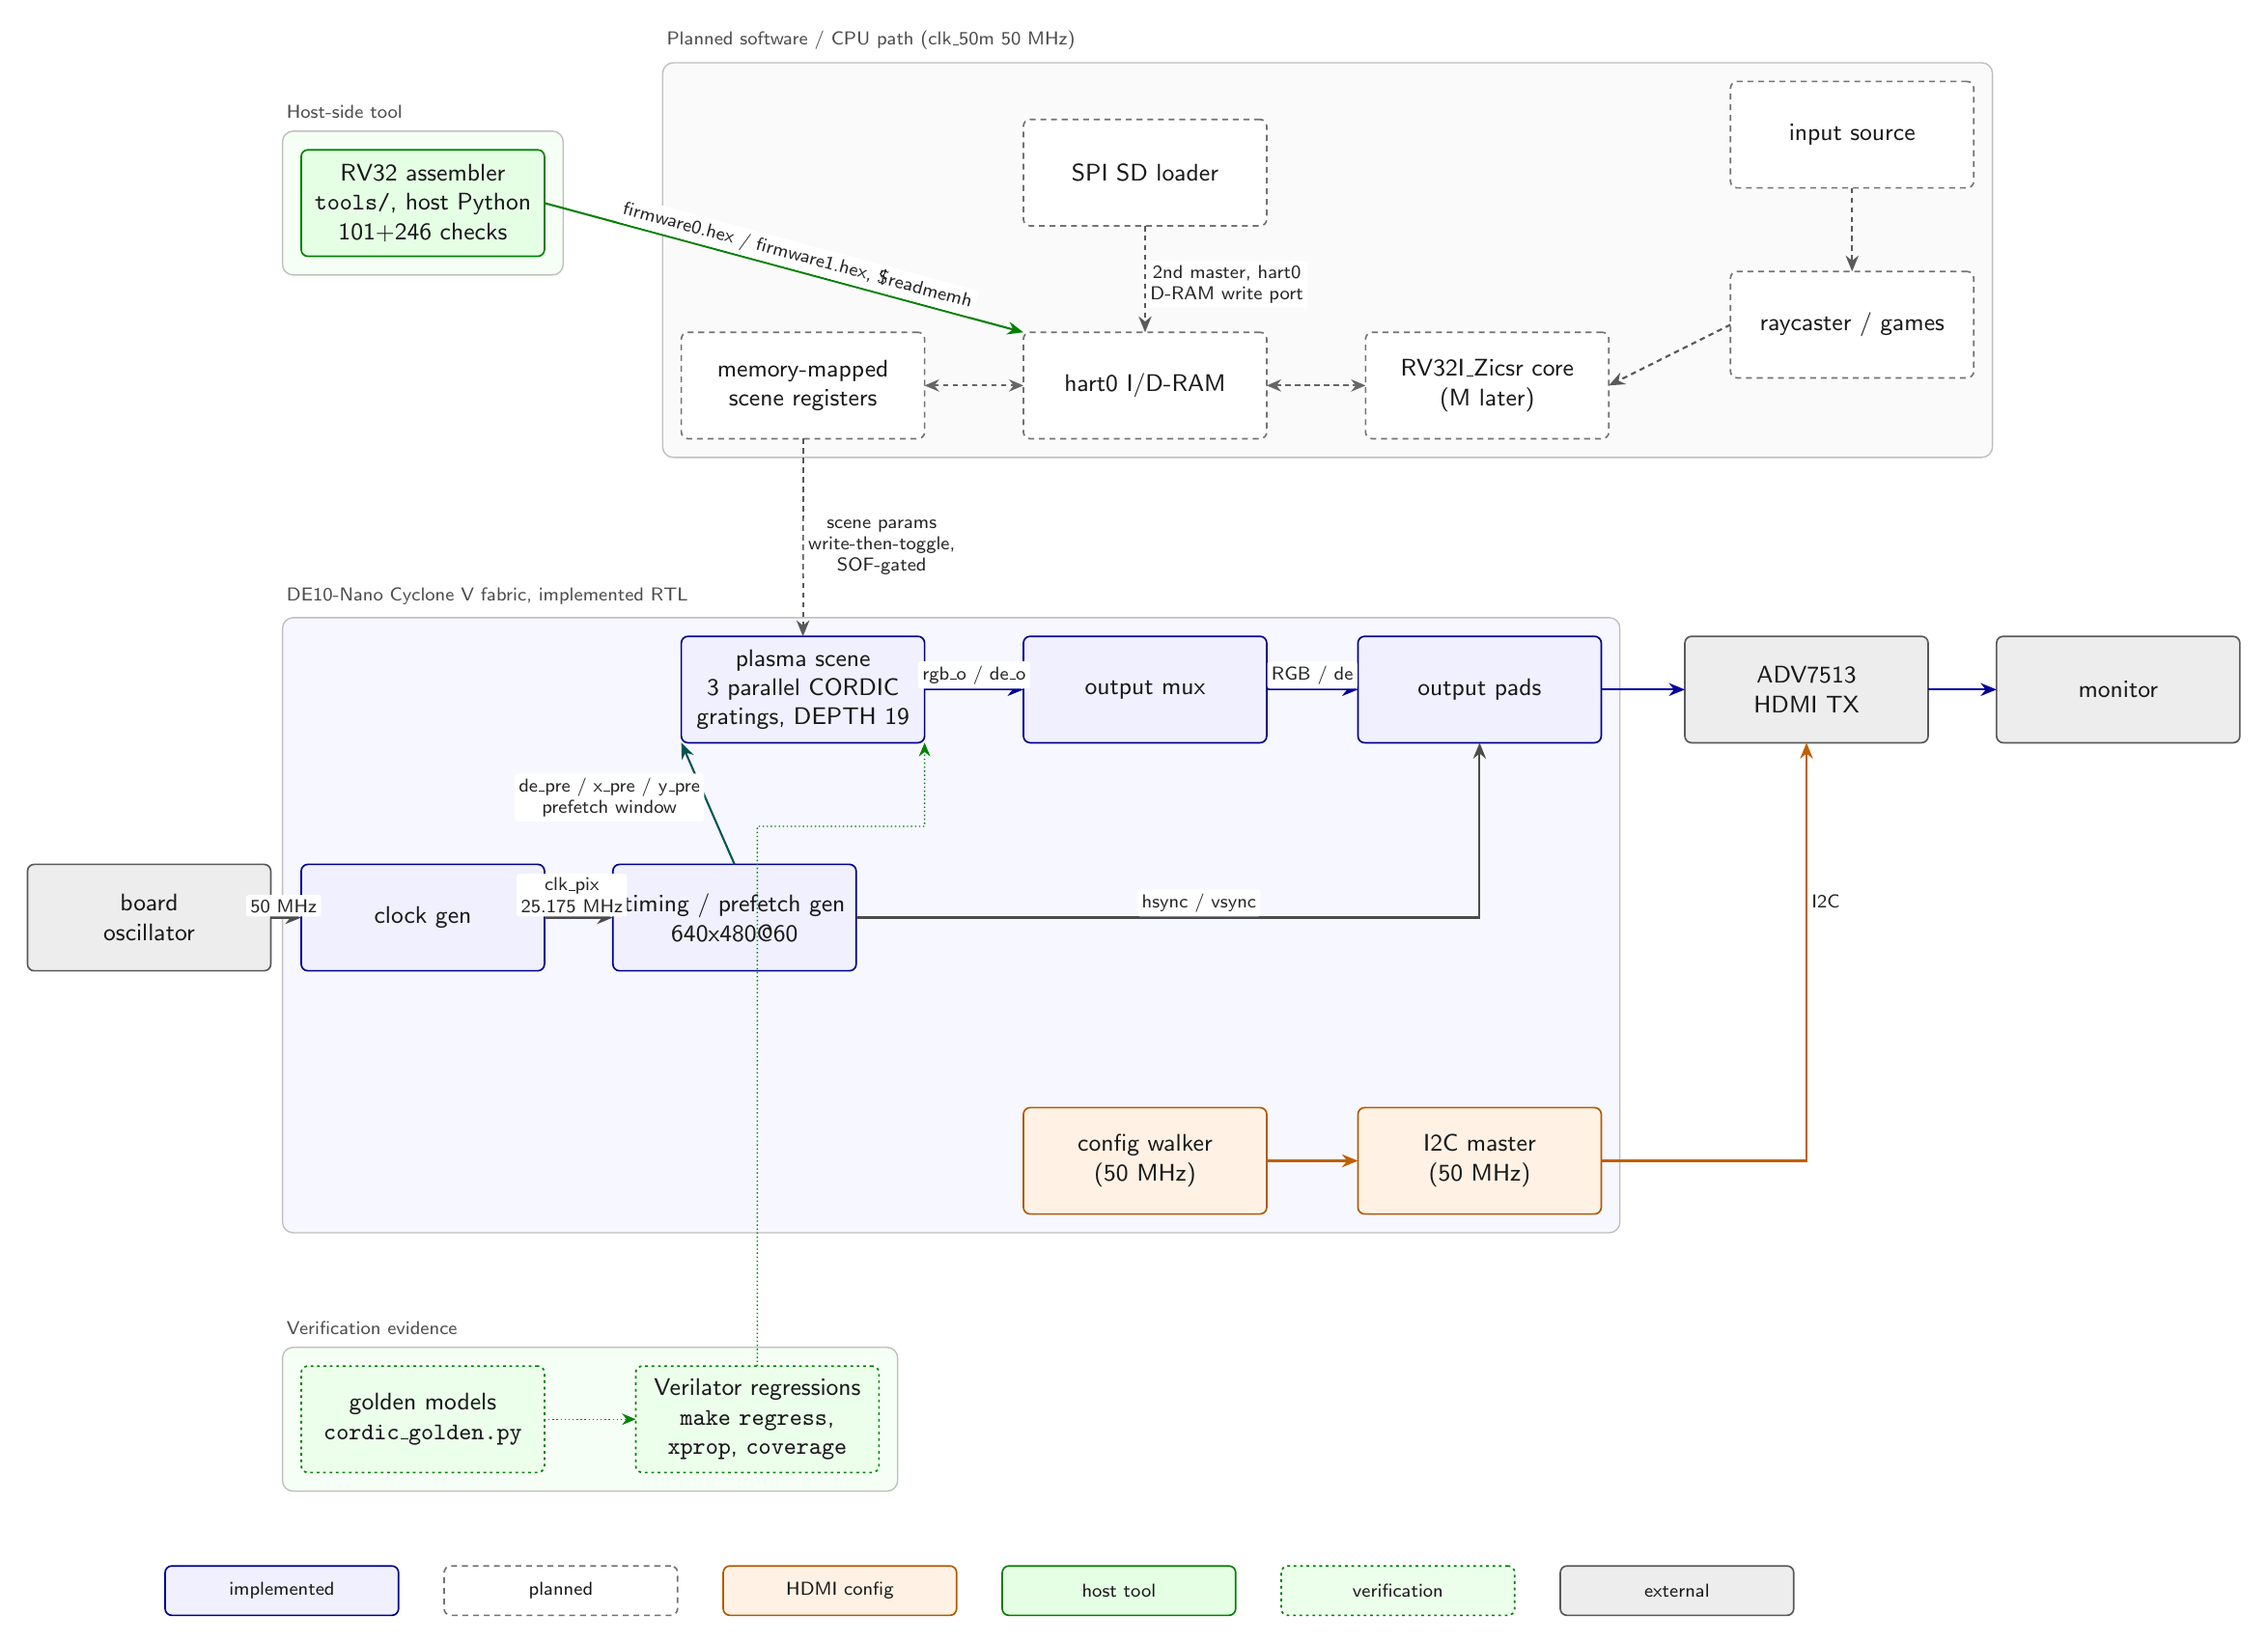
\begin{tikzpicture}[
  font=\sffamily\small,
  blk/.style={
    draw,
    rounded corners=2.5pt,
    line width=0.6pt,
    text width=30mm,
    minimum width=32mm,
    minimum height=14mm,
    align=center,
    inner sep=2.5pt,
    outer sep=0pt,
    text=black!90
  },
  impl/.style={blk, draw=blue!55!black, fill=blue!6},
  ext/.style={blk, draw=black!65, fill=black!7},
  ctrl/.style={blk, draw=orange!70!black, fill=orange!10},
  planned/.style={
    blk,
    draw=black!55,
    fill=white,
    dash pattern=on 2.2pt off 1.8pt
  },
  verif/.style={
    blk,
    draw=green!50!black,
    fill=green!8,
    dash pattern=on 1pt off 1.4pt
  },
  hostt/.style={blk, draw=green!50!black, fill=green!10},
  flow/.style={
    line width=0.75pt,
    -{Stealth[length=2.1mm,width=1.7mm]}
  },
  clkflow/.style={flow, black!70},
  pixel/.style={flow, blue!60!black},
  coord/.style={flow, teal!65!black},
  sync/.style={flow, black!70},
  ctrlflow/.style={flow, orange!75!black},
  planflow/.style={
    flow,
    black!65,
    dash pattern=on 2pt off 1.6pt
  },
  planbus/.style={
    black!60,
    line width=0.75pt,
    dash pattern=on 2pt off 1.6pt,
    {Stealth[length=1.9mm,width=1.6mm]}-{Stealth[length=1.9mm,width=1.6mm]}
  },
  loadflow/.style={flow, green!50!black},
  vdot/.style={
    -{Stealth[length=1.8mm,width=1.5mm]},
    green!50!black,
    line width=0.5pt,
    densely dotted
  },
  edgefont/.style={
    font=\scriptsize\sffamily,
    text=black!85,
    inner sep=1.6pt,
    fill=white,
    rounded corners=1pt,
    align=center
  },
  group/.style={
    draw=black!25,
    rounded corners=4pt,
    line width=0.5pt,
    inner sep=7pt
  },
  grouplabel/.style={
    font=\scriptsize\sffamily,
    text=black!70,
    fill=white,
    inner sep=1.6pt,
    rounded corners=1pt
  },
  legend/.style={
    minimum width=18mm,
    minimum height=6.5mm,
    font=\scriptsize\sffamily,
    inner sep=1pt,
    outer sep=0pt
  }
]

\node[impl] (plasma) at (0,3)
  {plasma scene\\3 parallel CORDIC\\gratings, DEPTH 19};

\node[impl] (mux) at (4.5,3)
  {output mux};

\node[impl] (pads) at (8.9,3)
  {output pads};

\node[ext] (adv) at (13.2,3)
  {ADV7513\\HDMI TX};

\node[ext] (mon) at (17.3,3)
  {monitor};

\node[ext] (osc) at (-8.6,0)
  {board\\oscillator};

\node[impl] (clk) at (-5.0,0)
  {clock gen};

\node[impl] (timing) at (-0.9,0)
  {timing / prefetch gen\\640x480@60};

\node[ctrl] (walker) at (4.5,-3.2)
  {config walker\\(50 MHz)};

\node[ctrl] (i2c) at (8.9,-3.2)
  {I2C master\\(50 MHz)};

\node[planned] (regs) at (0,7.0)
  {memory-mapped\\scene registers};

\node[planned] (mem) at (4.5,7.0)
  {hart0 I/D-RAM};

\node[planned] (core) at (9.0,7.0)
  {RV32I\_Zicsr core\\(M later)};

\node[planned] (sd) at (4.5,9.8)
  {SPI SD loader};

\node[planned] (games) at (13.8,7.8)
  {raycaster / games};

\node[planned] (inp) at (13.8,10.3)
  {input source};

\node[hostt] (asm) at (-5.0,9.4)
  {RV32 assembler\\\texttt{tools/}, host Python\\101+246 checks};

\node[verif] (oracle) at (-5.0,-6.6)
  {golden models\\\texttt{cordic\_golden.py}};

\node[verif] (veril) at (-0.6,-6.6)
  {Verilator regressions\\\texttt{make regress},\\
   \texttt{xprop}, \texttt{coverage}};

\draw[clkflow] (osc) -- node[edgefont, above, pos=0.42] {50 MHz} (clk);
\draw[clkflow] (clk) -- node[edgefont, above, pos=0.4] {clk\_pix\\25.175 MHz} (timing);

\draw[pixel] (plasma)
  -- node[edgefont, above] {rgb\_o / de\_o}
  (mux);

\draw[pixel] (mux)
  -- node[edgefont, above] {RGB / de}
  (pads);

\draw[pixel] (pads) -- (adv);
\draw[pixel] (adv) -- (mon);

\draw[coord] (timing.north)
  -- node[edgefont, left, pos=0.55]
     {de\_pre / x\_pre / y\_pre\\prefetch window}
  (plasma.south west);

\draw[sync] (timing.east)
  -- node[edgefont, above, pos=0.55]
     {hsync / vsync}
  (8.9,0)
  -- (pads.south);

\draw[ctrlflow] (walker) -- (i2c);

\draw[ctrlflow] (i2c.east)
  -- (13.2,-3.2)
  -- node[edgefont, right, pos=0.62]
     {I2C}
  (adv.south);

\draw[planbus] (regs) -- (mem);
\draw[planbus] (mem) -- (core);

\draw[planflow] (sd)
  -- node[edgefont, right, pos=0.55]
     {2nd master, hart0\\D-RAM write port}
  (mem);

\draw[planflow] (inp) -- (games);
\draw[planflow] (games.west) -- (core.east);

\draw[planflow] (regs.south)
  -- node[edgefont, right, pos=0.55]
     {scene params\\write-then-toggle,\\SOF-gated}
  (plasma.north);

\draw[loadflow] (asm.east)
  -- node[edgefont, above, sloped, pos=0.52]
     {firmware0.hex / firmware1.hex, \$readmemh}
  (mem.north west);

\draw[vdot] (oracle) -- (veril);

\draw[vdot] (veril.north)
  -- (-0.6,1.2)
  -- (1.6,1.2)
  -- (plasma.south east);

\begin{pgfonlayer}{background}
  \node[
    group,
    fill=blue!3,
    fit=(clk)(timing)(plasma)(mux)(pads)(walker)(i2c)
  ] (fabric) {};

  \node[
    group,
    fill=gray!4,
    fit=(regs)(mem)(core)(sd)(games)(inp)
  ] (plannedsw) {};

  \node[
    group,
    fill=green!4,
    fit=(asm)
  ] (hostgrp) {};

  \node[
    group,
    fill=green!4,
    fit=(oracle)(veril)
  ] (verifgrp) {};
\end{pgfonlayer}

\node[grouplabel, anchor=south west]
  at ($(fabric.north west)+(0,1mm)$)
  {DE10-Nano Cyclone V fabric, implemented RTL};

\node[grouplabel, anchor=south west]
  at ($(plannedsw.north west)+(0,1mm)$)
  {Planned software / CPU path (clk\_50m 50 MHz)};

\node[grouplabel, anchor=south west]
  at ($(hostgrp.north west)+(0,1mm)$)
  {Host-side tool};

\node[grouplabel, anchor=south west]
  at ($(verifgrp.north west)+(0,1mm)$)
  {Verification evidence};

\node[impl, legend] (l1)
  at ($(verifgrp.south west)+(0,-13mm)$)
  {implemented};

\node[planned, legend, right=6mm of l1] (l2)
  {planned};

\node[ctrl, legend, right=6mm of l2] (l3)
  {HDMI config};

\node[hostt, legend, right=6mm of l3] (l4)
  {host tool};

\node[verif, legend, right=6mm of l4] (l5)
  {verification};

\node[ext, legend, right=6mm of l5] (l6)
  {external};

\end{tikzpicture}
\end{document}
